\documentclass[twocolumn, 10pt]{article} % 全局字体大小设为12pt

% 导入 ctex 包以支持中文
\usepackage[UTF8]{ctex}
\usepackage{courier} % 用于设置代码字体

% 设置页面边距
\usepackage{geometry}
\geometry{left=2cm,right=2cm,top=2.5cm,bottom=2.5cm}
\usepackage{amsthm}

\usepackage{listings} % 用于显示代码
\usepackage{color}
\usepackage{algorithm}
\usepackage{algorithmic}




% 自定义带编号且斜体内容的 remark 环境
\theoremstyle{remark}
\newtheorem{remark}{Remark}

% 通过\textit命令让内容显示为斜体
\newenvironment{myremark}
  {\begin{remark}\itshape}
  {\end{remark}}


% 其他常用包
\usepackage{graphicx}   % 插入图片
\usepackage{amsmath}    % 数学公式
\usepackage{amssymb}    % 数学符号
\usepackage{hyperref}   % 超链接
\usepackage{enumitem}   % 引入 enumitem 包用于自定义列表
\usepackage{array} % 提供表格增强功能
\usepackage{stfloats} % 支持双栏排版中的浮动对象


\usepackage{xcolor} % 用于设置文本和背景颜色
\usepackage{times} % 设置全局字体为 Times New Roman,或者根据需求选择其他字体
% 表格字体设置
\usepackage{etoolbox}

% 导入titlecaps宏包
\usepackage{titlecaps}

\definecolor{codegray}{rgb}{0.5,0.5,0.5}
\definecolor{codeblue}{rgb}{0.25,0.5,0.75}
\definecolor{codepurple}{rgb}{0.58,0,0.82}

\lstdefinestyle{mystyle}{
    backgroundcolor=\color{white},   
    commentstyle=\color{codegray},
    keywordstyle=\color{codeblue},
    numberstyle=\tiny\color{codegray},
    stringstyle=\color{codepurple},
    basicstyle=\ttfamily\scriptsize, % 调整代码字体大小为 \scriptsize
    breakatwhitespace=false,         
    breaklines=true,                 
    captionpos=b,                    
    keepspaces=true,                 
    numbers=left,                    
    numbersep=5pt,                  
    showspaces=false,                
    showstringspaces=false,
    showtabs=false,                  
    tabsize=2
}

\lstset{style=mystyle}


% 自定义命令将标题首字母大写,其他单词小写
\Addlcwords{a an the of and in on at to with by for from}
\newcommand{\capitalizeTitle}[1]{\titlecap{#1}}

% 设置标题格式
\usepackage{titlesec}
\titleformat{\section}
  {\normalfont\Large\bfseries}
  {\thesection}{1em}{\capitalizeTitle}

\titleformat{\subsection}
  {\normalfont\large\bfseries}
  {\thesubsection}{1em}{\capitalizeTitle}

\titleformat{\subsubsection}
  {\normalfont\normalsize\bfseries}
  {\thesubsubsection}{1em}{\capitalizeTitle}









\AtBeginEnvironment{tabular}{\small} % 将表格内字体设为比正文小1号


% 定义浅黄色
\definecolor{lightyellow}{rgb}{1.0, 1.0, 0.88}

\begin{document}

% 标题
\title{MInference 1.0: Accelerating Pre-filling for Long-Context LLMs via Dynamic Sparse Attention}
\author{SL LV}
\date{\today}
\maketitle
% 摘要

\section{摘要-MInference 1.0: 通过动态稀疏注意力加速长上下文LLM的预填充阶}

大型语言模型(LLM)的推理计算挑战仍然是其广泛部署的重大障碍,尤其是在提示长度不断增加的情况下。由于注意力计算的二次复杂性,处理包含100万词元提示的8B LLM在单个A100 GPU上的预填充阶段可能需要长达30分钟的时间。现有的加速预填充阶段的方法在应用于长上下文LLM时,通常无法保持令人满意的准确性或效率。

为了解决这一问题,我们引入了MInference(Million-tokens Inference),这是一种旨在加速长序列处理的稀疏计算方法。具体而言,我们识别出长上下文注意力矩阵中的三种独特模式——A形模式、垂直斜线模式和块稀疏模式——可以用于在GPU上进行高效稀疏计算。我们离线确定每个注意力头的最佳模式,并在推理过程中动态生成稀疏索引。通过模式和稀疏索引,我们通过优化的GPU内核执行高效的稀疏注意力计算,显著减少了长上下文LLM预填充阶段的延迟。

我们提出的技术可以直接应用于现有的LLM,无需对预训练设置或额外微调进行任何修改。通过在一系列下游任务(如InfiniteBench、RULER、PG-19和Needle In A Haystack)以及包括LLaMA-3-1M、GLM-4-1M、Yi-200K、Phi-3-128K和Qwen-2-128K等模型上进行评估,我们证明了MInference在保持准确性的同时,将A100上预填充的推理延迟最多减少了10倍。我们的代码可以在\href{https://aka.ms/MInference}{https://aka.ms/MInference}上获取。



\section{引言}

\begin{figure*}[ht]
    \centering
    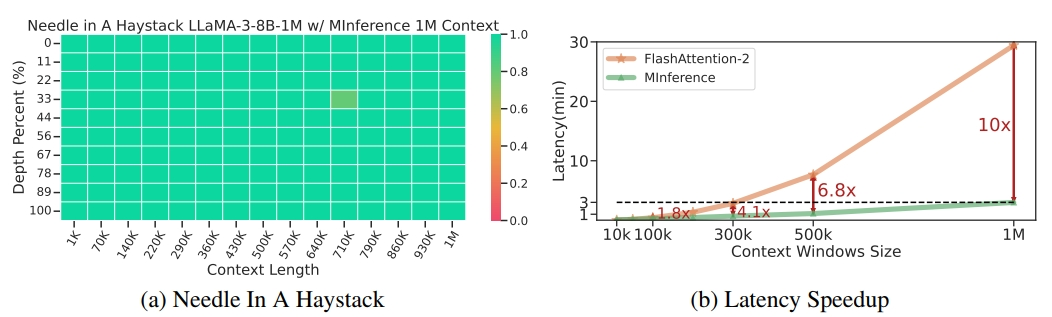
\includegraphics[width=0.8\textwidth]{m_attention_weights.png}
    \caption{
        这张图片展示了长上下文处理过程中注意力机制的动态稀疏性,并通过三个小图详细解释了相关内容:(a) 图表展示了在预填充阶段,注意力机制的计算代价随上下文窗口大小的增加而显著增加,最终成为主要的计算瓶颈;(b) 热力图展示了在128k上下文窗口中,前4k列所覆盖的注意力得分回忆率为96.4\%,表明注意力是稀疏的,大多数注意力得分集中在少数几个位置上;(c) 热力图展示了当前4k列应用于另一个128k上下文时,注意力得分回忆率下降到了83.7%,说明不同上下文之间的注意力稀疏模式是动态变化的。
    }
\end{figure*}


大型语言模型(LLMs)已经进入了长上下文处理的时代,其中一些模型支持从128K到1000万词元不等的上下文窗口。这些扩展上下文窗口使LLMs能够解锁许多复杂的实际应用,例如代码理解、长文档问答和长时间跨度的代理任务。

然而,由于注意力机制的二次复杂性,模型在处理输入提示(即预填充阶段)并开始生成第一个词元之前,可能需要几分钟的时间。例如,当在单个A100 GPU上为LLaMA-3-8B模型提供包含30万词元的提示时,模型需要6分钟才能完成预填充阶段,而当提示长度增加到100万词元时,这个时间增加到30分钟。自注意力计算的开销占据了总预填充延迟的90\%,这是长上下文处理的主要瓶颈。

为了应对这一挑战,本文提出了MInference,这是一种通过动态稀疏注意力计算减少95\%浮点运算(FLOPs)的技术,从而显著加速长上下文LLM推理的预填充阶段。与现有的动态稀疏注意力方法不同,MInference通过识别长上下文LLMs中三种独特的稀疏注意力模式——A形模式、垂直斜线模式和块稀疏模式——来减少计算开销。

基于这些发现,我们引入了一种内核感知搜索方法,用于在推理时为每个注意力头分配最佳模式。重要的是,与之前研究中使用的固定注意力掩码不同,我们采用了一种动态稀疏掩码,根据分配的模式和特定输入动态生成稀疏掩码。对于块稀疏模式,我们在64个块的基础上进行池化操作,并计算块级别的注意力权重,以确定最重要的块,并由此获得块稀疏动态掩码。

本文在多个长上下文LLM上进行了广泛的实验,包括LLaMA-3-8B、GLM-4-9B-1M和Yi-9B-200K,并使用了多个基准数据集,如InfiniteBench、RULER、PG-19和Needle In A Haystack。实验结果表明,MInference可以将LLaMA-3-8B模型在A100 GPU上的预填充延迟从30分钟减少到3分钟,同时保持或提高模型的准确性。


\section{Attention Heads: Dynamic, Sparse, and Characteristic}

\subsection{注意力机制的动态稀疏性}
\begin{figure*}[ht]
    \centering
    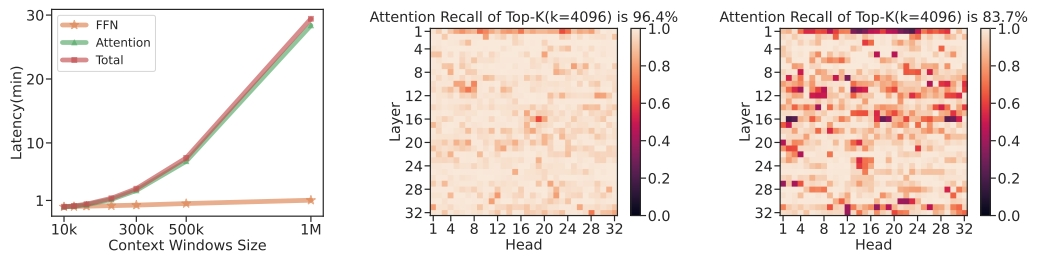
\includegraphics[width=0.8\textwidth]{m_latency_breakdown.png}
    \caption{
        这张图包含三个子图,展示了长上下文处理过程中注意力机制的动态稀疏性及其影响:(a) 显示了预填充阶段的延迟分解,随着上下文窗口大小的增加,注意力机制的计算代价显著增加,成为主要的计算瓶颈。橙色线表示前馈神经网络(FFN)的延迟,绿色线表示注意力机制的延迟,红色线表示总延迟;(b) 展示了在128k上下文中,前4k列所覆盖的注意力得分回忆率为96.4\%,说明注意力是稀疏的,绝大多数注意力得分集中在少数几个位置;(c) 当将(b)中的前4k列应用于另一个128k上下文时,注意力得分回忆率下降到了83.7\%,表明不同上下文之间的注意力稀疏模式具有动态变化的特性。这个结果基于在单个A100 GPU上运行的LLaMA-3-8B模型的可视化分析。
    }
\end{figure*}

预训练LLMs中的注意力权重稀疏性,尤其是在长上下文场景中,已被广泛记录。图2b所示的128k $\times$ 128k 的注意力矩阵中,仅保留前4k列就能回忆起96.8\%的总注意力。这意味着,尽管处理的序列较长,但每个词元实际上只关注了有限数量的词元。

然而,虽然不同输入的注意力矩阵中稀疏模式的自然特征是共享的,但这些稀疏模式的具体分布是高度动态的。换句话说,给定位置的词元在自注意力中只关注序列的一部分,且它关注的具体词元高度依赖上下文,并在不同提示间有显著差异。这种动态性在之前的研究中得到了数学上的验证。

图2c展示了如果将图2b中找到的前4k列应用于另一个128k的提示中,回忆注意力的比例将大幅下降至83.7\%。这表明,尽管稀疏模式可以在一定程度上被复用,但它们并非通用,且需要根据特定上下文动态调整。



\subsection{注意力稀疏性模式的展示}
\begin{figure*}[ht]
    \centering
    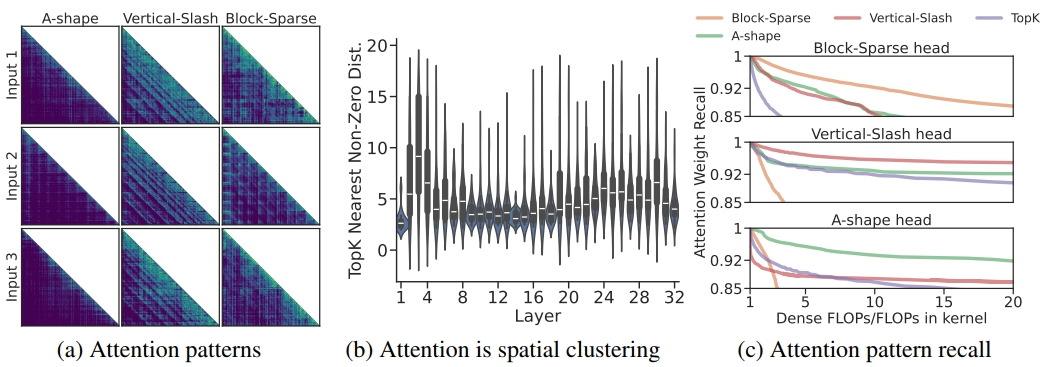
\includegraphics[width=0.8\textwidth]{visualization_of_attention_weights.png}
    \caption{
        这张图包含三个子图,展示了不同提示和任务下注意力头的稀疏模式及其对计算效率的影响:(a) 展示了不同输入下A形模式、垂直斜线模式和块稀疏模式的注意力权重可视化。相同注意力头的模式在不同输入下相对一致,但稀疏索引是动态变化的;(b) 展示了注意力矩阵中前10个最近非零元素的距离,显示了注意力权重的空间聚类特征。随着层数的增加,这种聚类特征变得更加明显;(c) 展示了使用识别出的模式计算注意力得分回忆率的分布情况。图中不同的曲线表示在不同的FLOPs配置下,不同稀疏模式的注意力权重回忆率。其中,块稀疏模式在最小化FLOPs的同时,能够较好地保持注意力权重回忆率,但随着FLOPs的增加,其表现可能会下降。所有可视化分析基于在LLaMA-3-8B-Instruct-262K模型上进行的实验结果。
    }
\end{figure*}

\begin{figure*}[ht]
    \centering
    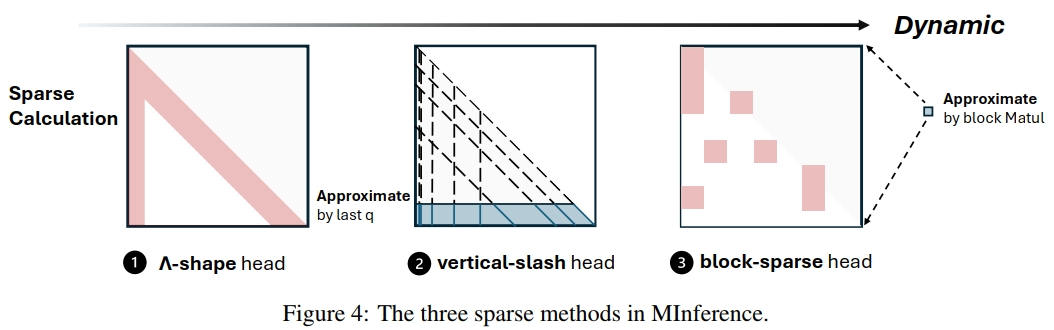
\includegraphics[width=0.8\textwidth]{the_three_sparse_methods_in_minference.png}
    \caption{
        图4展示了MInference中使用的三种稀疏计算方法: (1) \textbf{A形模式头}:该模式下的稀疏计算集中在初始和局部窗口内,计算量较小,适用于处理短期依赖; (2) \textbf{垂直斜线模式头}:通过最后一个查询词元(last q)的近似,稀疏计算沿着垂直和斜线分布,能够捕获较长范围的依赖; (3) \textbf{块稀疏模式头}:将注意力矩阵划分为块,进行块级别的稀疏计算,动态调整块的大小,适用于高效处理大规模上下文。三种模式从左到右逐渐增加动态性,以适应不同复杂性的计算需求。
    }
\end{figure*}


尽管注意力矩阵的稀疏分布是动态的,但先前的研究表明,它们在二维空间中表现出某些模式,例如空间聚类。本文通过分析不同长度提示的注意力分布,识别出了三种主要的稀疏模式:A形模式、垂直斜线模式(Vertical-Slash,VS)和块稀疏模式(Block-Sparse),如图3a和图4所示。表1详细描述了这些模式的特征和差异。

\paragraph{A形模式} 这种模式下的注意力权重主要集中在初始词元和局部窗口上,表现出相对较高的稳定性。

\paragraph{垂直斜线模式(VS)} 这种模式下的注意力权重集中在特定的词元(垂直线)和词元的分布(斜线)上。这些词元的分布随着上下文内容的变化而动态调整,并呈现出一定的稀疏性,使得这些模式难以被A形模式所涵盖。

\paragraph{块稀疏模式} 这种模式在不同上下文中具有高度动态性,同时表现出空间聚类的特征。在图3b中,我们展示了在128k上下文窗口中的前k个最近邻非零元素,词元之间的距离随着层数的增加而减小,表明注意力权重的空间聚类特征。

这三种稀疏模式能够实现高度高效的稀疏注意力计算,从而显著减少LLM推理中的计算成本(FLOPs)。图3c展示了这些稀疏模式在长上下文LLMs中的表现。具体而言,块稀疏模式在最小化FLOPs的同时,保持了较高的准确率。然而,对于Top-K注意力权重恢复,块稀疏模式表现出一定的挑战,因为它更关注全局的稀疏性,而其他模式则更专注于特定区域的稀疏性。


\section{MInference 1.0}
        在分析了第2节的内容之后,我们提出了MInference来加速长上下文LLMs的预填充阶段。MInference包括三个步骤:(1) 离线识别每个注意力头的注意力模式;(2) 根据模式动态生成稀疏索引;(3) 使用优化的GPU内核进行稀疏注意力计算。通过这三个步骤,MInference能够有效减少计算开销,加速推理过程。

\subsection{问题的形式化描述}

为了加速长上下文LLMs的预填充阶段的稀疏注意力计算,注意力矩阵可以表示为以下公式:
\[
A(M) = \text{Softmax}\left(\frac{1}{\sqrt{d}} QK^\top - c(1 - M)\right),
\]

其中,$M_{i,j} \in \{0, 1\}$ 表示注意力矩阵中第 $i, j$ 项的动态稀疏掩码。这里,$c$ 是一个大的常数,例如 $1e5$,确保对于那些 $M_{i,j} = 0$ 的不重要的注意力权重,在Softmax之后的值接近于零,即 $A_{i,j} \approx 0$。

动态稀疏注意力系统的目标是在尽可能保留注意力权重的同时,实现更大的加速,并最小化开销。形式化地,这可以表示为:
\[
\min \left|A(M) - A_{\text{dense}}\right|,
\]
\[
\min \ t_{\text{sparse}}(M) + t_{\text{overhead}}(M),
\]

其中,$t_{\text{sparse}}$ 和 $t_{\text{overhead}}$ 分别表示用于动态稀疏注意力计算和近似动态稀疏模式估计的时间。



\subsection{通过动态稀疏注意力加速长上下文LLM推理}
\begin{algorithm}[H]
\caption{Kernel-Aware Sparse Pattern Search}
\textbf{Input:} $Q, K, V \in \mathbb{R}^{S \times d_h}$, patterns $p$, search space $\rho$, target FLOPs $t$, initialized search space $\sigma$ \\
\textbf{Output:} Optimal pattern $p_{\text{best}}$

\textbf{\# Build kernel-aware search space}
\begin{algorithmic}[1]
\FOR{$i \gets 1$ \TO $|\sigma|$}
    \STATE $t_i \gets \text{FLOPs\_in\_kernel}(\sigma_i)$
    \WHILE{$|t_i - t| \geq \epsilon$}
        \STATE $\sigma_i \gets \text{ChangeSpace}(\sigma_i, \rho_i)$
        \STATE $t_i \gets \text{FLOPs\_in\_kernel}(\sigma_i)$
    \ENDWHILE
    \STATE $\rho \gets \rho \cup \sigma_i$
\ENDFOR

\textbf{\# Search for optimal head pattern}
\STATE $p_{\text{best}} \gets \phi$
\STATE $\psi \gets \text{Softmax}\left(\frac{Q K^\top}{\sqrt{d}}\right)$
\FOR{$i \gets 1$ \TO $|\rho|$}
    \STATE $y_i \gets \text{SparseAttention}\left(\frac{Q K^\top}{\sqrt{d}}, \rho_i\right)$
    \STATE $p_{\text{best}} \gets \text{argmin}(y_i - y_{p_{\text{best}}})$
\ENDFOR
\STATE \textbf{return} $p_{\text{best}}$
\end{algorithmic}
\end{algorithm}


\begin{algorithm}[H]
\caption{Vertical-Slash Head}
\textbf{Input:} $Q, K, V \in \mathbb{R}^{S \times d_h}$, $k_v, k_s \in \mathbb{N}$ \\
\textbf{Output:} Sparse attention output $y$

\textbf{\# Approximate vertical and slash pattern (last\_q = 64)}
\begin{algorithmic}[1]
\STATE $\hat{A} \gets \text{softmax}\left(\frac{Q_{[\text{-last\_q}]} K^\top}{\sqrt{d}} + m_{\text{casual}}\right)$

\textbf{\# Indices of top $k_v$ vertical line, sum in vertical}
\STATE $i_v \gets \text{argtopk}\left(\text{sum}_v(\hat{A}), k_v\right)$

\textbf{\# Indices of top $k_s$ slash line, sum in slash}
\STATE $i_s \gets \text{argtopk}\left(\text{sum}_s(\hat{A}), k_s\right)$

\textbf{\# Build sparse attention index}
\STATE $i_{vs} \gets \text{sparseformat}(i_v, i_s)$

\textbf{\# Final dynamic sparse attention scores (only index block)}
\STATE $A \gets \text{softmax}\left(\frac{\text{sparse}(Q K^\top, i_{vs})}{\sqrt{d}}\right)$

\textbf{\# Sparse mixed scores and values}
\STATE $y \gets \text{sparse}(A V, i_{vs})$

\STATE \textbf{return} $y$
\end{algorithmic}
\end{algorithm}


\begin{algorithm}[H]
\caption{Block-Sparse Head}
\textbf{Input:} $Q, K, V \in \mathbb{R}^{S \times d_h}$, $k_b \in \mathbb{N}$ \\
\textbf{Output:} Sparse attention output $y$

\textbf{\# Approximate block-sparse pattern (block\_size = 64)}
\begin{algorithmic}[1]
\STATE $\hat{Q} \gets \text{MeanPooling}(Q, \text{block\_size})$
\STATE $\hat{K} \gets \text{MeanPooling}(K, \text{block\_size})$
\STATE $\hat{A} \gets \text{softmax}\left(\frac{\hat{Q} \hat{K}^\top}{\sqrt{d}} + m_{\text{casual}}\right)$

\textbf{\# Indices of top $k$ blocks}
\STATE $i_b \gets \text{argtopk}(\hat{A}, k_b)$

\textbf{\# Build sparse attention index}
\STATE $i_b \gets \text{sparseformat}(i_b)$

\textbf{\# Final dynamic sparse attention scores (only index block)}
\STATE $A \gets \text{softmax}\left(\frac{\text{sparse}(Q K^\top, i_b)}{\sqrt{d}}\right)$

\textbf{\# Sparse mixed scores and values}
\STATE $y \gets \text{sparse}(A V, i_b)$

\STATE \textbf{return} $y$
\end{algorithmic}
\end{algorithm}


在这部分内容中,作者提出了内核感知的最优稀疏模式搜索方法,并进一步详细描述了稀疏索引近似和动态稀疏注意力计算。

\paragraph{内核感知的最优稀疏模式搜索}
为了在有限的FLOPs预算下达到最佳的模型精度,本文提出了离线内核感知最优稀疏模式搜索方法。该方法的第一步是为每个注意力头确定使用的稀疏模式,并选择该模式在实际计算中的最优设置(例如垂直斜线模式中的垂直线/斜线数量或块稀疏模式中的top-k块数)。作者通过目标FLOPs来定义搜索空间,并排除那些具有相似计算成本的候选模式。这个过程被称为“内核感知”,因为它反映了在GPU内核中实际消耗的FLOPs,而不仅仅是概念上的估计。

接下来,作者使用参考样本遍历整个搜索空间,以确定最佳模式和设置。这个过程的核心是以注意力矩阵的注意力得分回忆率作为搜索标准,从而确保在保留最大注意力权重的同时,最小化计算开销。最终,该方法使用FlashAttention来减少GPU内存开销,并实现端到端的最佳模式选择,从而进一步提升模型的推理效率。

\paragraph{稀疏索引近似与动态稀疏注意力计算}
在推理阶段,作者进一步探讨了如何在线估计注意力矩阵,以动态地确定稀疏性模式。具体来说,作者根据指定的模式和实际输入动态生成稀疏索引,并利用优化的GPU内核执行稀疏注意力计算。

(i) **垂直斜线头**:如算法2所示,由于垂直线和斜线的连续性,最后一个查询向量$Q_{\text{last\_q}}$与键向量$K$进行矩阵乘法,以生成估计的注意力矩阵$\hat{A}$。这进一步用于确定垂直线和斜线的稀疏索引$iv$和$is$。获得这些稀疏索引后,将它们转换为稀疏格式$ivs$,然后执行块稀疏的注意力权重和注意力输出计算。

(ii) **块稀疏头**:如算法3所述,首先对$Q$和$K$进行均值池化操作,以获得估计的块级注意力权重$\hat{A}$。然后,这些权重通过矩阵乘法操作与实际注意力权重的块稀疏模式进行近似,从而实现最小的计算开销。最终,通过构建稀疏索引$ib$并使用它来计算稀疏注意力权重和输出。

这些方法通过结合动态稀疏性,进一步优化了LLM在处理长上下文时的计算效率,显著减少了推理过程中的延迟。



\section{Experiments}

在这一部分中,我们探讨了 MInference 在长上下文 LLMs 中的有效性与效率性。具体来说,我们针对以下两个关键问题展开讨论:(i)MInference 的有效性如何?(ii)MInference 的效率如何?

\subsection{实验设置与基准测试}
实验中使用了四个最先进的长上下文 LLMs:LLaMA-3-8B-Instruct-262K、LLaMA-3-8B-Instruct-1048K、GLM-4-9B-1M 和 Yi-9B-200K。此外,我们还测试了 Needle In A Haystack 基准测试中的 Phi-3-Mini-128K 和 Qwen2-7B-128K。在实验中,我们使用了贪婪解码策略,确保结果的稳定性。实验代码基于 PyTorch 实现,并使用了 FlashAttention 和动态稀疏编译器 PIT。为实验设定的目标 FLOPs 是 1k 全局词元和 4k 局部窗口,在垂直斜线和块稀疏模式中分别设定 last\_q = 64 和 block\_size = 64。延迟实验在 Nvidia A100 GPU 上进行,使用 bfloat16 格式。

\subsection{数据集与评估指标}
我们使用了多个基准测试来评估 MInference 的有效性:

\begin{itemize}
    \item \textbf{InfiniteBench}:包含 10 项任务,包括信息检索、问题回答、摘要、代码调试等。平均上下文长度为 214K 词元。
    \item \textbf{RULER}:一个具有挑战性的长上下文基准测试,包含 13 项复杂任务,包括多跳追踪与聚合以及 QA 任务。上下文长度可达 128k 词元。
    \item \textbf{Needle In A Haystack}:用于测试 LLMs 在 1k 到 1M 词元范围内不同上下文窗口下的表现。
\end{itemize}

\subsection{基线方法与对比分析}
我们引入了五种基线方法作为对照:

\begin{itemize}
    \item \textbf{StreamingLLM with A-shape pattern}:使用 1k 全局词元和 4k 局部窗口。
    \item \textbf{StreamingLLM with dilated}:使用 1k 全局词元和 8k 稀疏局部窗口。
    \item \textbf{StreamingLLM with strided}:使用 1k 全局词元、2k 局部窗口和 4k 稀疏窗口。
    \item \textbf{InflLLM}:使用 128 全局词元和 8k 局部窗口。
    \item \textbf{我们的静态稀疏索引模式}:仅在预填充阶段进行稀疏计算,在解码阶段保持密集计算。
\end{itemize}

实验结果表明,在 InfiniteBench 基准测试中,MInference 在多个任务上超过了基线模型,尤其是在自然语言任务中,同时保持了模型的原始性能。此外,在检索相关任务中,MInference 的表现优于其他稀疏方法。

\subsection{特定基准测试的结果分析}

\paragraph{InfiniteBench} MInference 在总体表现上优于基线模型,甚至在某些任务上匹敌或略微超过了原始全注意力基线。我们的方法在自然语言任务中表现出色,例如摘要、问答和对话,同时在检索相关任务中也表现良好。

\paragraph{RULER} MInference 在复杂任务(如多跳追踪与聚合任务)中,能够有效维持长上下文性能,即使在测试长度超过 32K 的情况下,依然能够达到高效的上下文窗口效果。

\paragraph{Needle In A Haystack} MInference 能够在不同上下文窗口下有效地保留处理信息的能力,而基线模型(如 StreamingLLM)在超过临界信息量时性能快速下降。

\subsection{消融研究与延迟分析}
为了评估 MInference 各组件的重要性,我们进行了消融研究。实验结果表明,只有 A-shape 模式的静态方法在局部窗口内表现较差,而仅使用块稀疏模式或垂直斜线模式的版本虽然在动态性上有所平衡,但仍然落后于我们的方法。

延迟分析显示,MInference 在 100K、300K、500K 和 1M 词元上下文窗口下分别实现了 1.8x、4.1x、6.8x 和 10x 的加速效果。通过进一步利用张量并行和上下文并行技术,延迟可以减少到 8x A100 GPUs 上的 40 秒。

\subsection{KV 缓存压缩方法的集成}
我们还将 MInference 与先进的 KV 缓存压缩方法 SnapKV 结合使用。结果表明,大多数任务的性能几乎没有下降,进一步证明了 MInference 作为长上下文 LLMs 服务的优化策略的实际应用价值。


\section{论文创新点解析}

本论文在长上下文大型语言模型(LLM)推理的优化方面提出了多个关键的创新点,特别是在预填充阶段表现出显著的性能提升。以下是该论文的主要创新点的详细解析:

\subsection{动态稀疏注意力机制}
传统的稀疏注意力机制通常依赖于静态模式,无法适应上下文之间的动态变化。而该论文提出了一种动态稀疏注意力机制,可以根据输入数据的实际特征动态生成稀疏模式。这种方法显著减少了不必要的计算量,特别是在长上下文的处理过程中,降低了预填充阶段的计算开销。

\subsection{内核感知的稀疏模式搜索}
论文中介绍的内核感知稀疏模式搜索是一种离线方法,用于寻找在给定的计算预算下最优的稀疏模式。通过在内核层面进行搜索,该方法可以准确反映在GPU中实际执行的FLOPs,从而在稀疏模式选择时考虑到实际的计算成本。这一策略优化了计算效率,特别是在GPU资源有限的情况下,能够最大化推理的效率。

\subsection{稀疏索引的近似与构建}
该论文在动态稀疏计算中提出了两种主要的稀疏模式:垂直斜线模式和块稀疏模式。这些模式通过对注意力矩阵的关键部分进行重点计算,从而减少了整体的计算量。论文中提出的近似方法能够快速生成稀疏索引,并且这些索引能够动态适应不同的输入上下文,显著提升了模型的推理效率。

\subsection{多任务的基准测试}
论文通过在多个复杂任务上的基准测试来验证其方法的有效性。这些任务包括自然语言处理(如问答、摘要)以及代码调试等。MInference在这些任务上表现优异,特别是在处理长上下文时能够保持甚至超过传统全注意力机制的性能。这一结果证明了该方法不仅能够加速推理过程,还能在多个实际应用场景中保持模型的原有性能。

\subsection{与KV缓存压缩的集成}
该论文还探讨了将MInference与KV缓存压缩技术集成的可能性,并在实验中证明了这种集成能够在不显著影响性能的情况下进一步减少内存占用。通过这种集成,论文展示了在长上下文LLM推理中的一种高效、实用的优化路径。

\subsection{广泛的消融研究}
为了评估MInference各组件的作用,论文进行了广泛的消融研究。研究结果显示,动态稀疏策略的每个组件都在提高模型效率方面起到了至关重要的作用。尤其是当仅保留静态稀疏模式时,模型性能显著下降,进一步证明了动态稀疏策略的必要性和有效性。

通过这些创新,MInference在长上下文LLM推理中展示了显著的性能提升,特别是在预填充阶段大幅度减少了计算时间,提升了推理效率。这些方法不仅为学术研究提供了新的视角,也在实际应用中展现了巨大的潜力。


\end{document}
